\section{De volta ao sistema motivador}

%--------------------------------------------------------
\begin{frame}{Sistema hamiltoniano}
	Vamos relembrar o sistema trabalhado:
	\begin{equation*}
		H = \frac{1}{2}(q_1^2 + q_2^2 + q_1^2 q_2^2 + p_1^2 + p_2^2)
	\end{equation*}
	\begin{align*}
		\dot{q}_1 & = p_1, & \dot{p}_1 & = -q_1(1 + q_2^2), \\
		\dot{q}_2 & = p_2, & \dot{p}_2 & = -q_2(1 + q_1^2)  
	\end{align*}
\end{frame}

%--------------------------------------------------------
\begin{frame}{Operador e densidade}
	A evolução temporal é governada pelo operador de Liouville:
    \begin{equation*}
        L = p_1 \frac{\partial}{\partial q_1} - q_1(1 + q_2^2)\frac{\partial}{\partial p_1} + p_2 \frac{\partial}{\partial q_2} - q_2(1 + q_1^2)\frac{\partial}{\partial p_2}.
    \end{equation*}

	As variáveis não resolvidas seguem uma distribuição canônica com temperatura $T=1$:
	\begin{equation*}
		W(x) = \exp\left(\frac{-H(q,p)}{Z}\right)
	\end{equation*}
\end{frame}

%--------------------------------------------------------
\begin{frame}{Primeira aproximação: Modelo-$t$}
	Para simplificar o termo de memória, usamos a chamada aproximação modelo-$t$:
	\begin{equation*}
		\int_0^t e^{(t-s)L} \mathbb{P}L e^{s \mathbb{Q}L} ds \approx t e^{tL} \mathbb{P}L \mathbb{Q}L x_j
	\end{equation*}
	Chegamos à seguinte equação aproximada:
	\begin{equation*}
		\frac{d}{dt} e^{tL} \hat{x} = e^{tL} \mathbb{P}L \hat{x} + t e^{tL} \mathbb{P}L \mathbb{Q}L \hat{x} + e^{tL} \mathbb{Q}L \mathbb{Q}L x_j
	\end{equation*}
\end{frame}

%--------------------------------------------------------
\begin{frame}{Sistema com ruído}
	Com isso, as equações para $q_1$ e $p_1$ se tornam:
	\begin{align*}
		\frac{d}{dt} q_1 & = p_1,                                                                                                              \\
		\frac{d}{dt} p_1 & = -q_1\left(1 + \frac{1}{1 + q_1^2}\right) - 2t\frac{q_1^2 p_1}{(1 + q_1^2)^2} + e^{tL} \mathbb{Q}L \mathbb{Q}L p_1 
	\end{align*}
	O termo final representa o ruído originado pelas variáveis não resolvidas.
\end{frame}

%--------------------------------------------------------
\begin{frame}{Esperanças condicionais}
	Nosso objetivo é estimar:
	\begin{equation*}
		\mathbb{E}[q_1(t) | q_1(0), p_1(0)], \quad \mathbb{E}[p_1(t) | q_1(0), p_1(0)]
	\end{equation*}
	Ao aplicar o operador $\mathbb{P}$ às equações anteriores, o termo de ruído desaparece.
\end{frame}

%--------------------------------------------------------
\begin{frame}{Segunda aproximação}
	Adotamos uma segunda aproximação: comutação entre média e função.
	\begin{equation*}
		\mathbb{E}[(1 + q_1^2(t))^{-1} | q_1(0), p_1(0)] \approx \left(1 + \mathbb{E}[q_1(t)]^2\right)^{-1}
	\end{equation*}
	Com isso, definimos:
	\begin{equation*}
		Q_1(t) = \mathbb{E}[q_1(t)], \quad P_1(t) = \mathbb{E}[p_1(t)]
	\end{equation*}
\end{frame}

%--------------------------------------------------------
\begin{frame}{Sistema final}
	Finalmente, obtemos o sistema determinístico aproximado:
	\begin{align*}
		\frac{d}{dt} Q_1 & = P_1,                                                                                  \\
		\frac{d}{dt} P_1 & = -Q_1\left(1 + \frac{1}{1 + Q_1^2} \right) - t \cdot \frac{2 Q_1^2 P_1}{(1 + Q_1^2)^2} 
	\end{align*}
	Essa é a versão suavizada das equações iniciais, onde os efeitos do ruído foram absorvidos pela média.
\end{frame}

%--------------------------------------------------------

\begin{frame}{Gráfico}
	\begin{figure}[h]
		\centering
		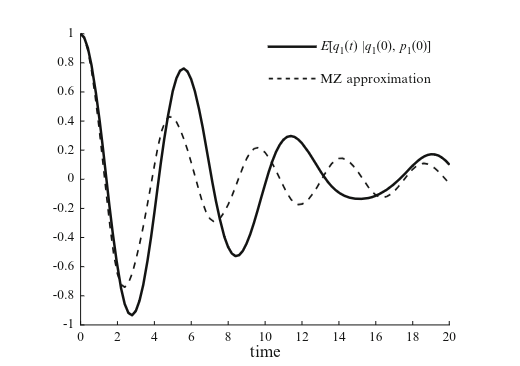
\includegraphics[width=0.4\textwidth]{03_SEMINARIO_MZ/02_APRESENTACAO/01_LATEX/img/grafico_motivacao_mz.png}
		\caption{Simulação - Exemplo motivador com o método Mori-Zwanzig}
		\label{fig:simulacao_exemplo_motivador_mz}
	\end{figure}
\end{frame}

